\documentclass[a4paper,11pt]{article}
\usepackage{amsmath,amsthm,amsfonts,amssymb,amscd,amstext,vmargin,graphics,graphicx,tabularx,multicol} 
\usepackage[francais]{babel}
\usepackage[utf8]{inputenc}  
\usepackage[T1]{fontenc} 
\usepackage{pstricks-add,tikz,tkz-tab,variations}
\usepackage[autolanguage,np]{numprint} 

\setmarginsrb{1.5cm}{0.5cm}{1cm}{0.5cm}{0cm}{0cm}{0cm}{0cm} %Gauche, haut, droite, haut
\newcounter{numexo}
\newcommand{\exo}[1]{\stepcounter{numexo}\noindent{\bf Exercice~\thenumexo} : \marginpar{\hfill /#1}}
\reversemarginpar


\newcounter{enumtabi}
\newcounter{enumtaba}
\newcommand{\q}{\stepcounter{enumtabi} \theenumtabi.  }
\newcommand{\qa}{\stepcounter{enumtaba} (\alph{enumtaba}) }
\newcommand{\initq}{\setcounter{enumtabi}{0}}
\newcommand{\initqa}{\setcounter{enumtaba}{0}}

\newcommand{\be}{\begin{enumerate}}
\newcommand{\ee}{\end{enumerate}}
\newcommand{\bi}{\begin{itemize}}
\newcommand{\ei}{\end{itemize}}
\newcommand{\bp}{\begin{pspicture*}}
\newcommand{\ep}{\end{pspicture*}}
\newcommand{\bt}{\begin{tabular}}
\newcommand{\et}{\end{tabular}}
\renewcommand{\tabularxcolumn}[1]{>{\centering}m{#1}} %(colonne m{} centrée, au lieu de p par défault) 
\newcommand{\tnl}{\tabularnewline}

\newcommand{\trait}{\noindent \rule{\linewidth}{0.2mm}}
\newcommand{\hs}[1]{\hspace{#1}}
\newcommand{\vs}[1]{\vspace{#1}}

\newcommand{\N}{\mathbb{N}}
\newcommand{\Z}{\mathbb{Z}}
\newcommand{\R}{\mathbb{R}}
\newcommand{\C}{\mathbb{C}}
\newcommand{\Dcal}{\mathcal{D}}
\newcommand{\Ccal}{\mathcal{C}}
\newcommand{\mc}{\mathcal}

\newcommand{\vect}[1]{\overrightarrow{#1}}
\newcommand{\ds}{\displaystyle}
\newcommand{\eq}{\quad \Leftrightarrow \quad}
\newcommand{\vecti}{\vec{\imath}}
\newcommand{\vectj}{\vec{\jmath}}
\newcommand{\Oij}{(O;\vec{\imath}, \vec{\jmath})}
\newcommand{\OIJ}{(O;I,J)}


\newcommand{\bmul}[1]{\begin{multicols}{#1}}
\newcommand{\emul}{\end{multicols}}

\newcommand{\reponse}[1][1]{%
\multido{}{#1}{\makebox[\linewidth]{\rule[0pt]{0pt}{20pt}\dotfill}
}}

\newcommand{\titre}[5] 
% #1: titre #2: haut gauche #3: bas gauche #4: haut droite #5: bas droite
{
\noindent #2 \hfill #4 \\
#3 \hfill #5

\vspace{-1.6cm}

\begin{center}\rule{6cm}{0.5mm}\end{center}
\vspace{0.2cm}
\begin{center}{\large{\textbf{#1}}}\end{center}
\begin{center}\rule{6cm}{0.5mm}\end{center}
}



\begin{document}
\pagestyle{empty}
\titre{Interrogation : Outils pour la physique}{Nom :}{Prénom :}{Classe}{Date}




\exo{2}  Cuáles son las gráficas donde la temperatura es proporcional al tiempo? (Justifica tu respuesta)\\

\includegraphics[scale=1.2]{graphiqueproporionnalite.eps} \\
\noindent \reponse[5]\\






\exo{2} Una familia fue de excursión a la montaña. El siguiente gráfico muestra la distancia recorrida en kilómetros versus el tiempo en horas.\\



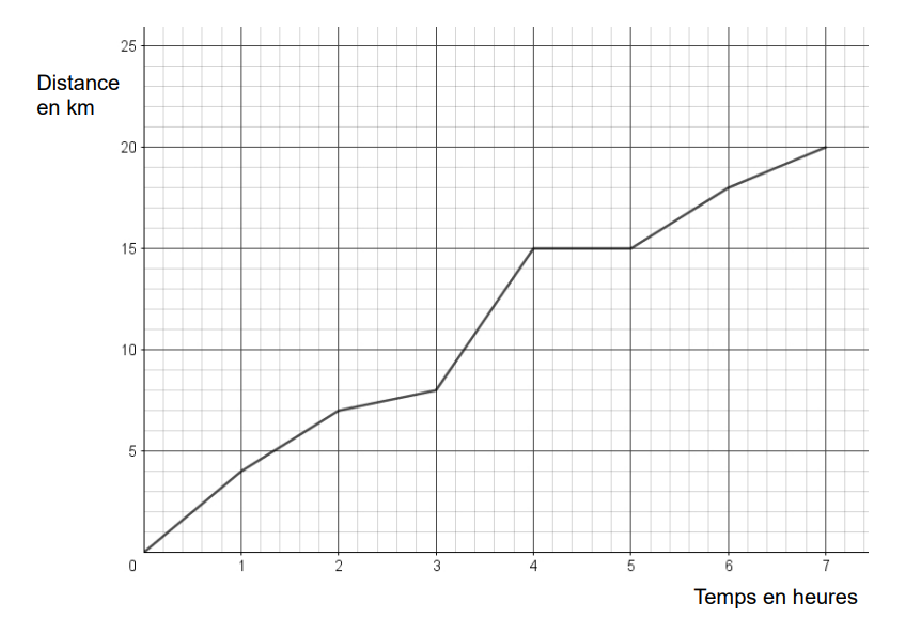
\includegraphics[scale=0.7]{graphiquelecture.eps} 
\initq



\textit{ Usaremos el gráfico para responder las siguientes preguntas. Ninguna justificación es solicitado.} \\
\q \qa Qué distancia viajó esta familia en total?\\
\reponse[1]\\

\qa Cuál es la distancia recorrida después de 6 horas de caminata?\\
\reponse[1]\\



\q Existe proporcionalidad entre la distancia recorrida y la duración de esta etapa? (Justifica tu respuesta)\\
\reponse[2]\\

\newpage

\exo{2} Una empresa produjo 300 toneladas de tuercas y tornillos. Vendió una cuarta parte de su producción en el mercado nacional, 50 \% en el mercado europeen, 10 \% en el mercado américano y el resto en el mercado asiático.\\

En cada caso, calcule la masa de nueces (en toneladas) vendidas.\\
\reponse[8]





\exo{1} Compléter avec l'écriture décimale ou bien la puissance de dix correspondante  :
\bmul{4}

$10^{3} = $ . . . . .

\columnbreak

. . . . . = 100

\columnbreak

$10^{8} = $ . . . . . 

\columnbreak

. . . . . = 10 000 

\emul





\exo{3} Aquí hay 4 objetos del universo:\\

\begin{tabular}{|c|c|c|c|}
\hline 
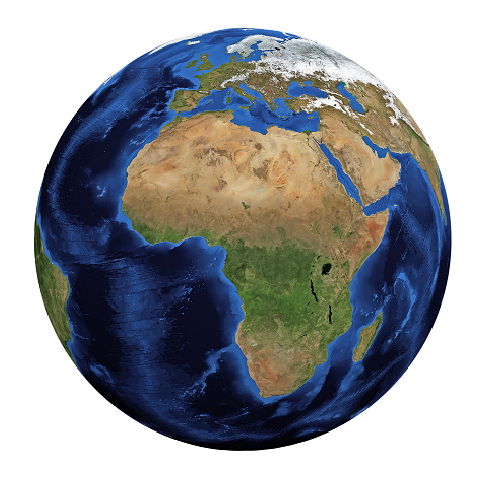
\includegraphics[scale=0.3]{terre.eps}  & 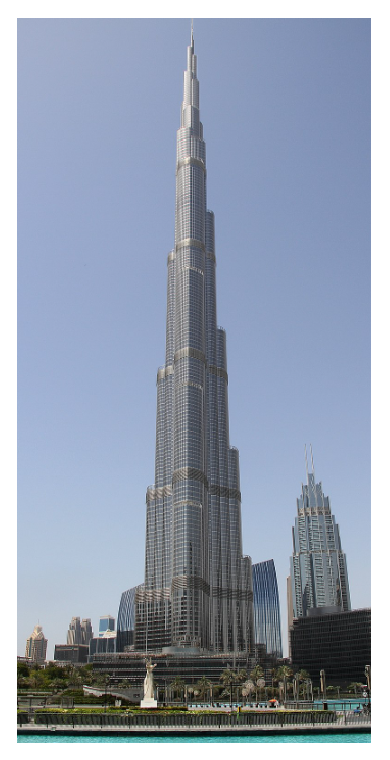
\includegraphics[scale=0.3]{tour.eps} & \includegraphics[scale=0.2]{galaxie.eps} & 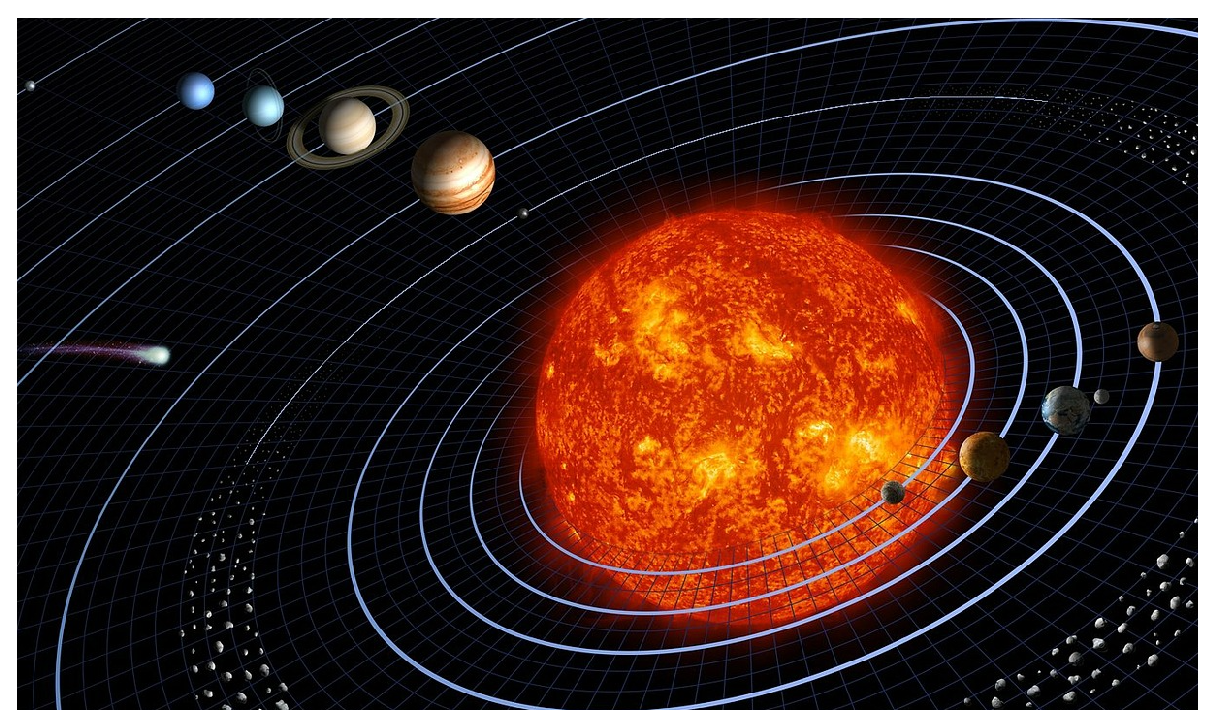
\includegraphics[scale=0.2]{systeme.eps}  \\ 
\hline 
La Terre & La plus haute tour du monde & La galaxie & Le système solaire  \\ 
\hline
\end{tabular} 


\vspace*{0.5cm}
Aquí están las dimensiones aproximadas de estos 4 objetos:\\

\begin{tabular}{|c|c|c|c|}
\hline 
\hspace*{0.5cm}828 m  \hspace*{0.5cm}& \hspace*{0.5cm}12 750 000 m \hspace*{0.5cm}&\hspace*{0.5cm} $ 12 \times 10^{12} $ m \hspace*{0.5cm}& \hspace*{0.5cm} $10^{21}$ m \hspace*{0.5cm}\\ 
\hline 
\end{tabular} 

\vspace*{0.5cm}
\initq 
\q Asocia cada objeto con su dimensión.\\
\reponse[4]\\

\q Pour pouvoir comparer des objets, les physiciens utilisent les distances en écriture scientifique.\\
Donner l'écriture scientifique de la dimension  de ces 4 objets.\\
\reponse[5]\\



\q Organice las dimensiones de estos objetos en orden ascendente.\\
\reponse[2]



\end{document}
